\section{Riesz's criterion and the Thorin path}\label{ch:riesz}

Section~\ref{wr:sec:riesz} introduced Riesz's criterion \cite{Riesz16} for the Riesz function \eqref{wr:eq:riesz} and its basepoint form, of which RH is the case $\alpha=\frac12$. Hardy and Littlewood \cite{HL16} gave a companion criterion with $\zeta(2k+1)$ in place of $\zeta(2k)$ and the exponent $-\frac14$, and the constructions of this section apply to it in the same way.

We develop the criterion in two directions. The first is computational (Section~\ref{ri:sec:filters}). The second reads the coefficients $1/\zeta(2k)$ through the clocks of Chapter~\ref{chap:basepoint}. None of this supplies the growth bound (Section~\ref{ri:sec:help}).

We keep the notation of Chapter~\ref{chap:basepoint} and Section~\ref{ch:strip} for $T=T_{1/2}$, $T_\alpha$, $\varphi_\alpha$, $H_a$, $b_\alpha$ and $v_\alpha$; in particular $b_1=\sum_\rho\rho^{-1}=0.0230957$. We write $\widetilde T=\widetilde T_1$ for the centre clock tilted by $e^{-T/4}$, as in Theorem~\ref{bp:thm:sub}, $\psi(y)=\sum_{n\le y}\Lambda(n)$ for Chebyshev's function, and
\[
\kappa_k=\frac{2k(2k-1)(k-1)!}{\pi^k},\qquad c_k=\frac1{\kappa_k\,\zeta(2k)},
\]
so that $\xi(2k)=\frac12\kappa_k\zeta(2k)$ and $c_k=\xi(1)/\xi(2k)$. The scripts named below are in \texttt{riesz\_program/code} of the archive, their outputs in \texttt{riesz\_program/data}.

\subsection{Which zeros the Riesz function sees}\label{ri:sec:filters}

On the range computed in Section~\ref{wr:sec:riesz} the Riesz function behaves exactly as RH predicts, and its fluctuations are accounted for by the known zeros, in fact by very few of them. In the explicit formula \eqref{wr:eq:rieszexplicit} a zero $\rho$ enters $R(x)$ through the term $r_\rho x^{\rho/2}$ with the weight $r_\rho=\Gamma(1-\rho/2)/(2\zeta'(\rho))$. By Stirling's formula $|\Gamma(\frac34-\frac i2\gamma)|$ decays like $e^{-\pi\gamma/4}$. The weight is $3.9\times10^{-5}$ for the first zero, whose term and that of its conjugate give the amplitude $7.8\times10^{-5}$ found in Section~\ref{wr:sec:riesz}, $2.1\times10^{-17}$ for the tenth, $1.5\times10^{-49}$ for the fiftieth and $2.2\times10^{-81}$ for the hundredth (\texttt{sens.py}, output \texttt{sens.json}; Figure~\ref{ri:fig:filters}, left). An off line zero at height $1000$ would enter with a weight near $10^{-340}$, and no feasible range of $x$ would reveal it. Riesz's criterion is equivalent to RH, but as a computational test it examines only the bottom of the spectrum.

The remedy is to change the kernel. For real $h$ put
\[
R_h(x)=x\sum_{n\ge1}\frac{\mu(n)}{n^2}\Big(\frac x{n^2}\Big)^{ih}e^{-x/n^2},\qquad x>0,
\]
so that $R_0=R$.

\begin{proposition}\label{ri:prop:twisted}
For every real $h$ and $\frac12<\re s<1$,
\[
\int_0^\infty R_h(x)\,x^{-s-1}dx=\frac{\Gamma(1-s+ih)}{\zeta(2s)} .
\]
For $\frac12\le\alpha<1$, $\zeta$ has no zeros in the half plane $\re s>\alpha$ if and only if $R_h(x)=O(x^{\alpha/2+\delta})$ for every $\delta>0$. In particular RH holds if and only if $R_h(x)=O(x^{1/4+\delta})$ for every $\delta>0$.
\end{proposition}

\begin{proof}
Term by term, $\int_0^\infty x^{1+ih}n^{-2-2ih}e^{-x/n^2}x^{-s-1}dx=n^{-2s}\Gamma(1-s+ih)$, and summing against $\mu(n)$ gives $\Gamma(1-s+ih)\sum_n\mu(n)n^{-2s}$; the interchange is justified because, with $\sigma=\re s$, the integrals of the absolute values sum to $\Gamma(1-\sigma)\zeta(2\sigma)<\infty$. Suppose that $\zeta$ has no zeros in $\re s>\alpha$. Then $1/\zeta(2s)$ is analytic in $\re s>\frac\alpha2$. By the argument of \cite[Section 14.2]{Titchmarsh} with the line of real part $\alpha$ in place of the critical line, as in Section~\ref{wr:sec:riesz}, $|1/\zeta(2s)|\le|2\im s|^{C_\delta}$ on $\re s\ge\frac\alpha2+\delta$, $|\im s|\ge5$, while $|\Gamma(1-s+ih)|$ decays like $e^{-\pi|\im s-h|/2}$ in vertical strips. So the Mellin inversion integral $R_h(x)=\frac1{2\pi i}\int_{(c)}\Gamma(1-s+ih)\zeta(2s)^{-1}x^s\,ds$, with $\frac12<c<1$, can be moved to the line $\re s=\frac\alpha2+\delta$, which gives $R_h(x)=O(x^{\alpha/2+\delta})$. Conversely, if $R_h(x)=O(x^{\alpha/2+\delta})$ as $x\to\infty$, then, since also $|R_h(x)|\le\zeta(2)\,x$, the Mellin integral converges absolutely for $\frac\alpha2+\delta<\re s<1$ and continues $\Gamma(1-s+ih)/\zeta(2s)$ analytically there. As $\Gamma$ has no zeros, $\zeta(2s)$ has no zeros with $\alpha+2\delta<\re2s<2$; since $\delta>0$ is arbitrary and $\zeta$ has no zeros with $\re s\ge1$, it has none with $\re s>\alpha$.
\end{proof}

Shifting the contour further gives, when the zeros are simple, the twisted form of the explicit formula \eqref{wr:eq:rieszexplicit}, with the sum over the zeros again the limit of its partial sums over $|\gamma|<T_\nu$ along a suitable sequence $T_\nu\to\infty$:
\begin{equation}\label{ri:eq:twexplicit}
R_h(x)=\sum_\rho\frac{\Gamma(1-\rho/2+ih)}{2\zeta'(\rho)}\,x^{\rho/2}+\sum_{k\ge1}\frac{\Gamma(1+k+ih)}{2\zeta'(-2k)}\,x^{-k}.
\end{equation}
The heights $T_\nu$ are those of \cite[Theorem 9.7]{Titchmarsh}, on which $1/\zeta(\sigma+iT_\nu)=O(T_\nu^A)$ for $-1\le\sigma\le2$; with the functional equation for $\re2s\le-1$ this makes the integrals over the horizontal segments $\im2s=\pm T_\nu$ tend to $0$. On the line $\re s=-q-\frac12$ we write $1/\zeta(2s)=\pi^{1/2-2s}\Gamma(s)/(\Gamma(\frac12-s)\zeta(1-2s))$; since $|\Gamma(1-s+ih)\Gamma(s)|\le e^{\pi|h|/2}\pi/\cosh(\pi\im s)$, $|\Gamma(\frac12-s)|\ge q!\,(\pi t/\sinh\pi t)^{1/2}$ with $t=\im s$, and $|\zeta(1-2s)|\ge2-\zeta(4)$, the integral over that line is at most $Ce^{\pi|h|/2}\pi^{2q}x^{-q-1/2}/q!$, which tends to $0$ as $q\to\infty$.

What the twist changes is the weight. Since $|\Gamma(\frac34+i(h-\gamma/2))|$ is largest when $\gamma\approx2h$ and decays like $e^{-\pi|h-\gamma/2|/2}$ away from it, $R_h$ sees the zeros in a band of width about ten around height $2h$. At $h=50$ the largest weight among the first $300$ zeros is $0.124$, at $\gamma=101.3$, where the untwisted weight is $2.9\times10^{-35}$ (Figure~\ref{ri:fig:filters}, left). With \texttt{twisted.py} we computed $R_{50}(x)$ from the M\"obius series with $\mu$ sieved to $10^7$ at forty values of $x$ in $[10^4,10^{10}]$, and compared it with \eqref{ri:eq:twexplicit} over the first $300$ zeros and three trivial terms. The two agree to $1.2\times10^{-8}$ in $|R_h(x)|/x^{1/4}$, against a signal of size up to $0.27$, and the zeros with $|\gamma-100|<15$ carry $99.9997\%$ of the modulus of the explicit formula, in the median over the forty values of $x$ (Figure~\ref{ri:fig:filters}, right).

An off line zero with real part $\beta$ near height $2h$ would contribute a term of size $x^{\beta/2}$, growing relative to the background $x^{1/4}$ by the factor $x^{(\beta-1/2)/2}$: a factor $3.2$ between $x=10^{10}$ and $x=10^{20}$ when $\beta=0.6$.

\begin{remark}\label{ri:rem:indep}
Twisted Riesz functions are not competitive with direct zero finding as a verification method. Their value is independence: they are computed from $\mu(n)$ only, with no evaluation of $\zeta$, so agreement between $R_h$ and the explicit formula over computed zeros is a check of the zeros that shares no code or method with their computation.
\end{remark}

The cost of $R(x)$ or $R_h(x)$ is dominated by sieving $\mu(n)$ to $N=K\sqrt x$. Terms with $n<\sqrt x/12$ are below $e^{-144}$ and can be omitted, and the terms with $n>N$ are summed through $\sum_n\mu(n)n^{-2}=6/\pi^2$, or $1/\zeta(2+2ih)$ for $R_h$: the script computes $R(x)/x$ as $\sum_{\sqrt x/12\le n\le N}\mu(n)n^{-2}e^{-x/n^2}+\big(6/\pi^2-\sum_{n\le N}\mu(n)n^{-2}\big)$, and the neglected remainder $\sum_{n>N}\mu(n)n^{-2}(e^{-x/n^2}-1)\approx-x\sum_{n>N}\mu(n)n^{-4}$ is of order $xN^{-7/2}$ under square root cancellation in the M\"obius tail, that is, of order $K^{-7/2}$ in $R(x)/x^{1/4}$. That cancellation is proved in the range used: the Mertens function $\sum_{n\le t}\mu(n)$ is less than $0.571\sqrt t$ in absolute value for $33\le t\le10^{16}$ \cite[Section 6.1]{Hurst18}, and partial summation then bounds the remainder in $R(x)/x^{1/4}$ by $1.1\times10^{-8}$ for $K=200$ and $1\le x\le10^{12}$. The script \texttt{riesz\_large.py} implements this with a segmented sieve and extended precision. With $K=200$ it reproduces the explicit formula over $60$ zeros and three trivial terms to about $2\times10^{-9}$ in $R(x)/x^{1/4}$ at $x=10^8$, $10^{10}$, $10^{11}$ and $10^{12}$ (\texttt{check\_large.py}). Its twisted option agrees as well: at $x=10^{10}$ with $h=50$ it gives $R_{50}(x)=37.441416-26.042495\,i$, within $3.1\times10^{-9}$ of \eqref{ri:eq:twexplicit} over $300$ zeros in $|R_h(x)|/x^{1/4}$ (\texttt{check\_large\_twisted.py}).

\begin{figure}[htbp]
\centering
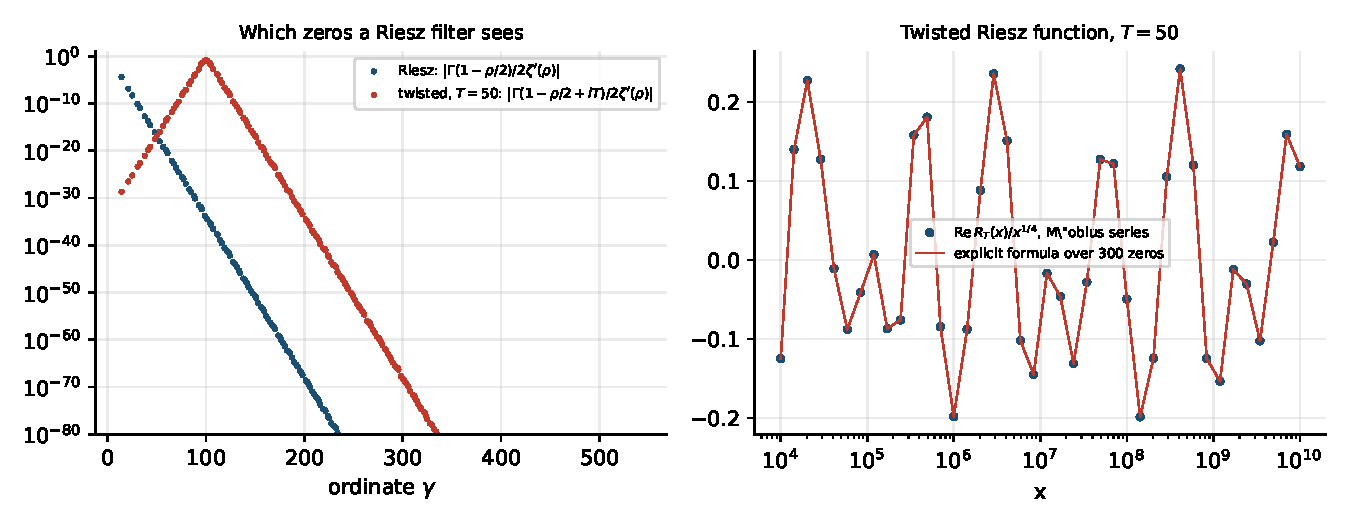
\includegraphics[width=\textwidth]{fig/ri_filters.pdf}
\caption{Left: the weights $|\Gamma(1-\rho/2)/(2\zeta'(\rho))|$ of the Riesz function and $|\Gamma(1-\rho/2+ih)/(2\zeta'(\rho))|$ of the twisted Riesz function with $h=50$, for the first $300$ zeros. Right: $\re R_{50}(x)/x^{1/4}$ from the M\"obius series against the explicit formula \eqref{ri:eq:twexplicit} over $300$ zeros. The plot writes $T$ for $h$. Data from \texttt{twisted.py}; drawn by \texttt{figs\_strategy.py}.}
\label{ri:fig:filters}
\end{figure}

\subsection{The Riesz coefficients through the centre clock}\label{ri:sec:thorin}

The Riesz coefficients are values of two Laplace transforms: that of the centre clock $T$ of \cite{P17} and that of the basepoint one clock $T_1$ (Proposition~\ref{bp:prop:thorin}).

\begin{proposition}\label{ri:prop:coef}
For every integer $k\ge1$, with no hypothesis,
\[
\frac1{\zeta(2k)}=\frac{\kappa_k}{2\xi(\frac12)}\;\E\,e^{-(2k-\frac12)^2T}=\kappa_k\;\E\,e^{-(2k-1)^2T_1}.
\]
\end{proposition}

\begin{proof}
From the definition of $\xi$, $\xi(2k)=k(2k-1)\pi^{-k}\Gamma(k)\zeta(2k)=\frac12\kappa_k\zeta(2k)$. Since $2k-\frac12>0$, the Laplace transform of $T$ at $(2k-\frac12)^2$ is $\varphi_{1/2}((2k-\frac12)^2)=\xi(\frac12)/\xi(2k)$; similarly $\E e^{-(2k-1)^2T_1}=\xi(1)/\xi(2k)$, with $\xi(1)=\frac12$.
\end{proof}

\begin{proposition}\label{ri:prop:avg}
For every $x>0$, with no hypothesis,
\[
R(x)=-\frac1{\xi(\frac12)}\;\E\Big[\sum_{k\ge1}k(2k-1)\Big(-\frac x\pi\Big)^ke^{-(2k-\frac12)^2T}\Big].
\]
\end{proposition}

\begin{proof}
Since $\kappa_k/(2(k-1)!)=k(2k-1)\pi^{-k}$, Proposition~\ref{ri:prop:coef} turns the term $-(-x)^k/((k-1)!\,\zeta(2k))$ of Riesz's series into $-\xi(\frac12)^{-1}k(2k-1)(-x/\pi)^k\,\E e^{-(2k-\frac12)^2T}$. The exchange of sum and expectation is justified by Fubini's theorem, because
\[
\sum_{k\ge1}k(2k-1)\Big(\frac x\pi\Big)^k\E\,e^{-(2k-\frac12)^2T}=\xi(\tfrac12)\sum_{k\ge1}\frac{x^k}{(k-1)!\,\zeta(2k)}<\infty .
\]
\end{proof}

The terms of the series averaged in Proposition~\ref{ri:prop:avg} decay like $e^{-4k^2T}$ rather than like $1/(k-1)!$. Table~\ref{ri:tab:check}, computed by \texttt{riesz\_thorin.py} (output \texttt{riesz\_thorin.json}), checks both propositions with $4\times10^5$ draws of $T$, generated under RH as $\sum_{\gamma>0}e_\gamma/\gamma^2$ with independent standard exponentials $e_\gamma$: the first $200$ zeros are used exactly, and the remaining terms are replaced by a gamma variable with the same mean and variance, computed from the exact power sums $\sum\gamma^{-2}$ and $\sum\gamma^{-4}$. The coefficients agree within about one standard error, and so do the values of $R$ from the M\"obius series, the power series and the clock average.

\begin{table}[htbp]
\centering\small
\begin{tabular}{cccc}
\toprule
$k$ & $1/\zeta(2k)$ & via the clock & standard error\\
\midrule
1 & 0.6079271 & 0.6079115 & 0.0000131\\
2 & 0.9239384 & 0.9238153 & 0.0001046\\
3 & 0.9829526 & 0.9826581 & 0.0002603\\
4 & 0.9959392 & 0.9954609 & 0.0004615\\
\bottomrule
\end{tabular}
\qquad
\begin{tabular}{cccc}
\toprule
$x$ & $R(x)$, M\"obius & clock average & standard error\\
\midrule
0.5 & 0.1252199 & 0.1252287 & 0.0000074\\
1 & 0.0439818 & 0.0440007 & 0.0000157\\
2 & $-0.2677934$ & $-0.2677918$ & 0.0000026\\
5 & $-0.7705597$ & $-0.7706050$ & 0.0000397\\
\bottomrule
\end{tabular}
\caption{Left: the Riesz coefficients from the clock, Proposition~\ref{ri:prop:coef}. Right: the Riesz function from the M\"obius series, which agrees with the power series to fourteen digits, and from the clock average of Proposition~\ref{ri:prop:avg}.}
\label{ri:tab:check}
\end{table}

The clock average is also far better conditioned than the power series. Riesz's power series is numerically hopeless for large $x$: its largest term is about $e^x\sqrt{x/2\pi}$, that is $10^{4344.5}$ at $x=10^4$, while $R(10^4)$ is of order $10^{-3}$. In the clock average the largest term of the inner series, $\max_kk(2k-1)(x/\pi)^ke^{-(2k-\frac12)^2T}$, is about $10^{81}$ at $x=10^4$ for the typical value $T=0.023$, and its logarithm grows like $(\log x)^2/(16T)$ instead of like $x$ (Figure~\ref{ri:fig:riesz}, right).

\begin{figure}[htbp]
\centering
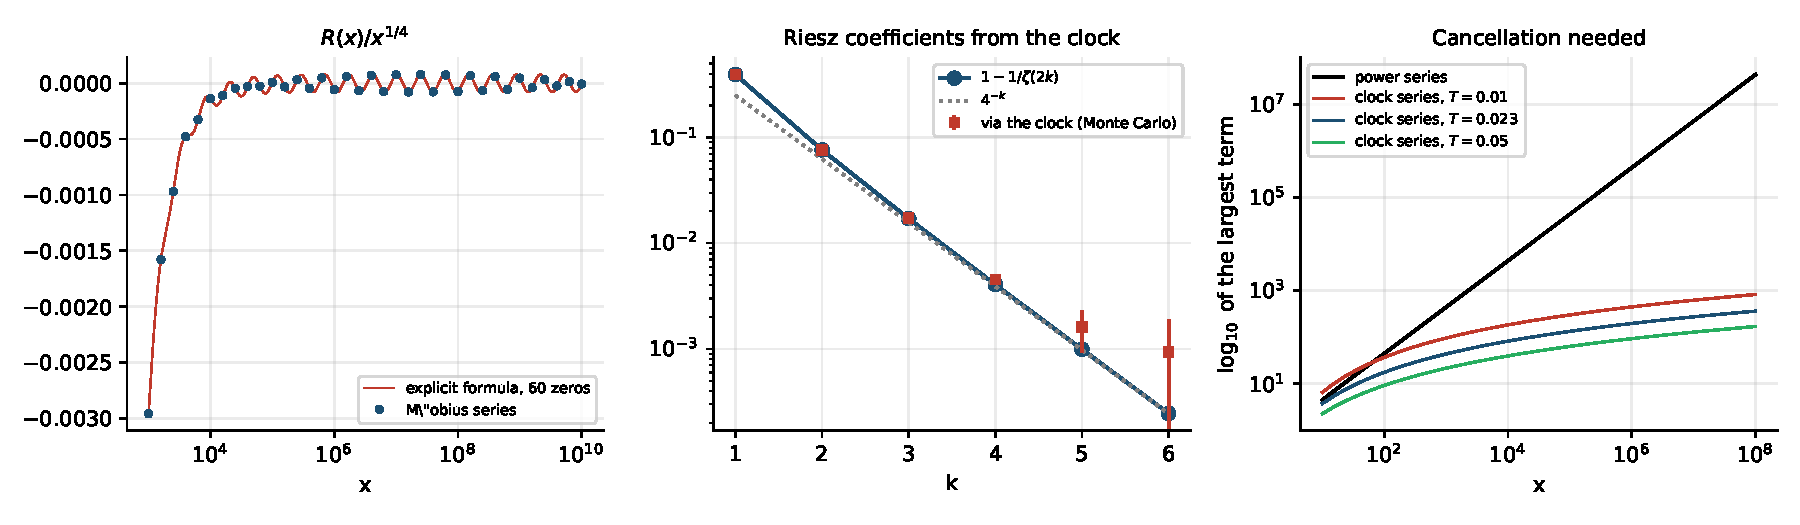
\includegraphics[width=\textwidth]{fig/ri_riesz.pdf}
\caption{Left: $R(x)/x^{1/4}$ from the M\"obius series and from the explicit formula over $60$ zeros, as in the right panel of Figure~\ref{wr:fig:salem}. Middle: $1-1/\zeta(2k)$ and its Monte Carlo value from the clock (Proposition~\ref{ri:prop:coef}), against $4^{-k}$. Right: base ten logarithm of the largest term in Riesz's power series and in the clock series of Proposition~\ref{ri:prop:avg} for $T=0.01$, $0.023$ and $0.05$.}
\label{ri:fig:riesz}
\end{figure}

\subsection{The sine squared lemma and a GGC form of Riesz's criterion}\label{ri:sec:ggc}

The computation of Proposition~\ref{ri:prop:coef} works at every basepoint between the centre and one. For $\alpha>\frac12$ the clock $T_\alpha$ exists with no hypothesis (Theorem~\ref{bp:thm:alpha}), and it is a GGC exactly when $\zeta$ has no zeros with $\re s>\alpha$ (Theorem~\ref{thm:poisson}).

\begin{proposition}[Riesz coefficients as GGC values]\label{ri:prop:ggccoef}
For every $\alpha\in[\frac12,1]$ and every integer $k\ge1$,
\[
\frac1{\zeta(2k)}=\frac{\kappa_k}{2\xi(\alpha)}\;\E\,e^{-(2k-\alpha)^2T_\alpha}.
\]
At $\alpha=1$, with no hypothesis, $T_1$ is a GGC with Thorin density $\rho_{1/2}=v_1/\pi$ in the chart $\theta=\sqrt z$, and
\[
\frac1{\zeta(2k)}=\kappa_k\exp\Big\{-\int_0^\infty\log\Big(1+\frac{(2k-1)^2}{\theta^2}\Big)\rho_{1/2}(\theta)\,d\theta\Big\}.
\]
\end{proposition}

\begin{proof}
Since $2k-\alpha>0$, the Laplace transform of $T_\alpha$ at $(2k-\alpha)^2$ is $\xi(\alpha)/\xi(2k)$, and $\xi(2k)=\frac12\kappa_k\zeta(2k)$. At $\alpha=1$, $\xi(1)=\frac12$, and the Thorin representation $\log\varphi_1(u)=-\int_0^\infty\log(1+u/\theta^2)\rho_{1/2}(\theta)\,d\theta$ of Proposition~\ref{bp:prop:thorin}, taken at $u=(2k-1)^2$, gives the second formula.
\end{proof}

\begin{remark}\label{ri:rem:hcm}
All the Riesz coefficients are samples of one GGC Laplace transform: $c_k=\varphi_1((2k-1)^2)$, where $\varphi_1(u)=\E e^{-uT_1}$. As a Laplace transform $\varphi_1$ is completely monotone, and this already makes $\log\varphi_1$ convex in $u$, by H\"older's inequality; so the slopes $(\log c_{k+1}-\log c_k)/8k$ increase with $k$. As the transform of a GGC, $\varphi_1$ is also hyperbolically completely monotone \cite[Theorem 6.1.1]{Bondesson}: for each $u>0$ the function $v\mapsto\varphi_1(uv)\varphi_1(u/v)$ is a completely monotone function of $v+1/v$. In particular it decreases as $v$ moves away from $1$, and differentiating $\log\varphi_1(uv)+\log\varphi_1(u/v)$ in $\log v$ shows that $t\mapsto\log\varphi_1(e^t)$ is concave. At the sample points this gives inequalities in the other direction: the slopes $(\log c_{k+1}-\log c_k)/\log\frac{2k+1}{2k-1}$ decrease with $k$, and $c_jc_l\le c_k^2$ whenever $(2j-1)(2l-1)=(2k-1)^2$, for instance $c_1c_5\le c_2^2$.
\end{remark}

The Thorin density $v_1/\pi$ is built from the primes by the sine squared lemma \eqref{eq:sin2}. Proposition~\ref{bp:prop:levy} writes $\log(\xi(1+s)/\xi(1))$ in the L\'evy form \eqref{bp:eq:levyform}, with the drift $b_1$ and a signed L\'evy measure $\Pi_1$ made of the gamma density, the pole of $\zeta$ and the prime atoms, and the lemma converts it term by term into the Thorin form $v_1=b_1+A+Q$ of \eqref{bp:eq:conversion}, with the gamma piece $A$ and the compensated prime piece $Q$. The L\'evy form in $s=2k-1$ is
\[
\frac1{\zeta(2k)}=\kappa_k\exp\Big\{-b_1(2k-1)-\int_0^\infty\big(e^{-(2k-1)x}-1+(2k-1)x\big)\,\Pi_1(dx)\Big\},
\]
and in the Thorin form in $u=(2k-1)^2$ the drift splits off a positive stable one half factor:
\begin{equation}\label{ri:eq:factor}
\frac1{\zeta(2k)}=\kappa_k\;e^{-b_1(2k-1)}\;\exp\Big\{-\frac1\pi\int_0^\infty\log\Big(1+\frac{(2k-1)^2}{\theta^2}\Big)\big(A(\theta)+Q(\theta)\big)\,d\theta\Big\}.
\end{equation}
This is the factorisation $T_1\stackrel d=S+T_1^\circ$ of Proposition~\ref{bp:prop:v1min} evaluated at $u=(2k-1)^2$: the middle factor is $\E e^{-(2k-1)^2S}$ for the positive stable variable $S$ of index one half with $\E e^{-uS}=e^{-b_1\sqrt u}$, and the last factor is $\E e^{-(2k-1)^2T_1^\circ}$ for the independent GGC $T_1^\circ$ with Thorin density $(A+Q)/\pi=(v_1-b_1)/\pi$.

Inserting Proposition~\ref{ri:prop:ggccoef} at $\alpha=1$ into the power series gives the Riesz function as a GGC mixture,
\begin{equation}\label{ri:eq:mixture}
R(x)=-2\,\E\Big[\sum_{k\ge1}k(2k-1)\Big(-\frac x\pi\Big)^ke^{-(2k-1)^2T_1}\Big],
\end{equation}
where the exchange of sum and expectation is justified as in Proposition~\ref{ri:prop:avg}, since $\sum_k2k(2k-1)(x/\pi)^kc_k=\sum_kx^k/((k-1)!\,\zeta(2k))<\infty$. The variable $T_1$ has two realisations. It is the tilted centre clock run through the inverse local time of a sticky Brownian motion (Theorem~\ref{bp:thm:sub} and the paragraph after it), and, like every GGC without drift \cite{JRY}, it is the Wiener gamma integral \eqref{pm:eq:wg} against the inverse of the Poisson smoothed zero count $M_{1/2}(\theta)=\pi^{-1}\int_0^\theta v_1$ (Section~\ref{pm:sec:wg}).

\begin{theorem}\label{ri:thm:ggcriesz}
For $\frac12\le\alpha<1$ the following are equivalent:
\begin{enumerate}
\item $R(x)=O(x^{\alpha/2+\delta})$ for every $\delta>0$;
\item $\zeta$ has no zeros with $\re s>\alpha$;
\item $T_{\alpha'}$ is a GGC for every $\alpha'>\alpha$;
\item for every $\alpha'>\alpha$, $v_{\alpha'}(\theta)=\re\frac{\xi'}\xi(\alpha'+i\theta)\ge0$ at every real $\theta$ for which $\alpha'+i\theta$ is not a zero of $\xi$;
\item for every $\alpha'>\alpha$ and every real $\theta$ the compensated sine squared sum
\[
\lim_{L\to\infty}\Big[\sum_{\log n\le L}\frac{\Lambda(n)}{n^{\alpha'}}\,2\sin^2\Big(\frac{\theta\log n}2\Big)-\int_0^L2\sin^2\Big(\frac{\theta x}2\Big)e^{(1-\alpha')x}\,dx\Big]
\]
converges.
\end{enumerate}
In particular RH holds if and only if $T_\alpha$ is a GGC for every $\alpha>\frac12$.
\end{theorem}

\begin{proof}
Write $\Theta=\sup\re\rho$ and $D(y)=\psi(y)-y$. Conditions (1) and (2) are equivalent by the basepoint version of Riesz's criterion (Section~\ref{wr:sec:riesz}, and Proposition~\ref{ri:prop:twisted} with $h=0$). Conditions (2) and (3) are equivalent by Theorem~\ref{thm:poisson}: $\varphi_{\alpha'}$ is the Laplace transform of a GGC exactly when $\alpha'\ge\Theta$, and this holds for every $\alpha'>\alpha$ exactly when $\Theta\le\alpha$, which is (2).

(2) implies (4), because if $\Theta\le\alpha<\alpha'$ every Cauchy kernel in $v_{\alpha'}(\theta)=\sum_\rho(\alpha'-\beta)/((\alpha'-\beta)^2+(\theta-\gamma)^2)$ has positive width (Proposition~\ref{prop:struct}). Conversely, let $\rho_0=\beta_0+i\gamma_0$ be a zero of multiplicity $m$ with $\beta_0>\alpha$. The zeros of $\xi$ are isolated, so only finitely many lie on the segment $\{\sigma+i\gamma_0:0\le\sigma\le1\}$. Let $n_0$ be the number of those other than $\rho_0$, counted with multiplicity, and choose $\eta\in(0,\beta_0-\alpha)$ with $|\beta-\beta_0|\ge2\eta$ for each of them. For $\alpha'\in(\beta_0-\eta,\beta_0)$ the point $\alpha'+i\gamma_0$ is not a zero, and Proposition~\ref{prop:struct} gives
\[
v_{\alpha'}(\gamma_0)=\frac m{\alpha'-\beta_0}+\sum_{\rho\ne\rho_0,\ \gamma=\gamma_0}\frac1{\alpha'-\beta}+\sum_{\gamma\ne\gamma_0}\frac{\alpha'-\beta}{(\alpha'-\beta)^2+(\gamma-\gamma_0)^2}.
\]
The middle sum is at most $n_0/\eta$ in absolute value. Since $\alpha'$ and $\beta$ lie in $(0,1)$, each term of the last sum is at most $(\gamma-\gamma_0)^{-2}$ in absolute value, and $\sum_{\gamma\ne\gamma_0}(\gamma-\gamma_0)^{-2}<\infty$: finitely many zeros have $0<|\gamma-\gamma_0|<1$, and for $|\gamma-\gamma_0|\ge1$ we have $(\gamma-\gamma_0)^{-2}\le5/(4+(\gamma-\gamma_0)^2)\le5(2-\beta)/((2-\beta)^2+(\gamma-\gamma_0)^2)$, a series bounded by $5v_2(\gamma_0)<\infty$. Hence $v_{\alpha'}(\gamma_0)\le m/(\alpha'-\beta_0)+n_0/\eta+\sum_{\gamma\ne\gamma_0}(\gamma-\gamma_0)^{-2}<0$ for $\alpha'$ close to $\beta_0$, and (4) fails at $(\alpha',\gamma_0)$.

(2) implies (5). This is part 1 of Proposition~\ref{bp:prop:below} at the basepoint $\alpha'$, since $\Theta\le\alpha<\alpha'$, and the argument is short. Choose $\sigma$ with $\Theta<\sigma<\alpha'$, so that $D(y)=O(y^\sigma)$ \cite{Titchmarsh}. With $f(y)=y^{-\alpha'}\,2\sin^2(\frac12\theta\log y)$ the bracket in (5) is
\[
\int_{(1,e^L]}f\,dD=f(e^L)D(e^L)-\int_1^{e^L}D(y)f'(y)\,dy,
\]
since $f(1)=0$. The boundary term tends to $0$, and the integral converges absolutely because $|f'(y)|\le(2\alpha'+|\theta|)y^{-\alpha'-1}$.

(5) implies (2). Suppose (5), and let $\rho_0$ be a zero of multiplicity $m$ with $\re\rho_0>\alpha$. Fix $\alpha'\in(\alpha,\re\rho_0)$ and $\theta\notin\mathcal E=\{\theta:\rho_0+i\theta\text{ or }\rho_0-i\theta\text{ is a zero}\}$, a countable set that contains $0$, and let $M(t)=\int_{(0,t]}(1-\cos\theta s)\,dD(e^s)$, a function of locally bounded variation. The bracket in (5) is $J(L)=\int_{(0,L]}e^{-\alpha't}dM(t)$; by hypothesis it converges as $L\to\infty$, so $J$ is bounded. For $\re w>\alpha'$, integration by parts gives
\[
\int_{(0,L]}e^{-wt}\,dM(t)=e^{-(w-\alpha')L}J(L)+(w-\alpha')\int_0^Le^{-(w-\alpha')t}J(t)\,dt,
\]
which converges as $L\to\infty$, locally uniformly in $w$, to an analytic function $F_\theta(w)$ on $\re w>\alpha'$. For $\re w>1$ the integral converges absolutely, and writing $1-\cos\theta t=1-\frac12e^{i\theta t}-\frac12e^{-i\theta t}$ gives
\begin{gather*}
F_\theta(w)=g(w)-\tfrac12g(w-i\theta)-\tfrac12g(w+i\theta),\\
g(w)=\int_{(1,\infty)}y^{-w}\,dD(y)=-\frac{\zeta'}\zeta(w)-\frac1{w-1}.
\end{gather*}
The right side, call it $\widetilde F_\theta(w)$, is meromorphic in the plane with a discrete set $\mathcal P$ of poles. On the connected open set $\Omega=\{\re w>\alpha'\}\setminus\mathcal P$ both $\widetilde F_\theta$ and $F_\theta$ are analytic, and they agree on $\re w>1$, so $\widetilde F_\theta=F_\theta$ on $\Omega$ by the identity theorem. The function $g$ is analytic at $1$, and in $\re w>0$ its only poles are the zeros of $\zeta$, each simple with residue minus its multiplicity. Since $\theta\notin\mathcal E$, $g(w\pm i\theta)$ is analytic at $\rho_0$, so $\widetilde F_\theta$ has a pole at $\rho_0$ with residue $-m\ne0$, and $|F_\theta(w)|\to\infty$ as $w\to\rho_0$ in $\Omega$. This contradicts the continuity of $F_\theta$ at $\rho_0$, where $\re\rho_0>\alpha'$. Hence no zero has real part greater than $\alpha$, which is (2).
\end{proof}

\subsection{The coefficients as killing probabilities}\label{ri:sec:kill}

For a positive random variable $X$ and an independent exponential variable $E_\lambda$ of rate $\lambda$, $\E e^{-\lambda X}=P(X<E_\lambda)$, the probability that $X$ occurs before a killing at rate $\lambda$. Propositions~\ref{ri:prop:coef} and \ref{ri:prop:ggccoef} therefore say that every Riesz coefficient is a killing probability, in two ways and with no hypothesis:
\begin{equation}\label{ri:eq:kill}
\frac1{\zeta(2k)}=\kappa_k\,P\big(T_1<E_{(2k-1)^2}\big)=\frac{\kappa_k}{2\xi(\frac12)}\,P\big(T<E_{(2k-\frac12)^2}\big).
\end{equation}
By Theorem~\ref{bp:thm:sub}, $T_1\stackrel d=\widetilde T+H_{\widetilde T/\sqrt2}$, and by the paragraph after it $T_1$ is the first time the local time at zero of a sticky Brownian motion exceeds an independent level distributed as $\widetilde T$. So $c_k=1/(\kappa_k\zeta(2k))$ is the probability that this hitting happens before an independent killing at rate $(2k-1)^2$.

The factorisation \eqref{ri:eq:factor} has the same reading. Since $\E e^{-\lambda H_a}=e^{-a\sqrt{2\lambda}}$, the stable factor is
\[
e^{-b_1(2k-1)}=P\big(H_{b_1/\sqrt2}<E_{(2k-1)^2}\big),
\]
the probability that Brownian motion reaches the level $b_1/\sqrt2=0.016331$ before it is killed. So $S\stackrel d=H_{b_1/\sqrt2}$ and $T_1\stackrel d=H_{b_1/\sqrt2}+T_1^\circ$ with $T_1^\circ$ an independent GGC. Thus $c_k=P(H_{b_1/\sqrt2}<E_{(2k-1)^2})\,P(T_1^\circ<E'_{(2k-1)^2})$, with independent exponential clocks $E$ and $E'$ of the same rate. If the exact Brownian boundary $b$ of $T_1$ is bounded at infinity, as Section~\ref{bp:sec:rs1} observes but does not prove, Lemma~\ref{bp:lem:wald} and the tail of $T_1$ make the level $b_1/\sqrt2=\sum_\rho\rho^{-1}/\sqrt2$ its Wald defect $\E\,b(T_1)$.

Under RH, if the zeros are also simple, more is true. The centre clock is then a GGC with unit atoms at the distinct points $\gamma^2$ (Proposition~\ref{prop:rigid}), hence, by Kent's theorem and Krein's inverse spectral theory (Section~\ref{sec:ch18:kent}), the hitting time of a level by the diffusion of a Krein string with Dirichlet spectrum $\{\gamma^2\}$ (Table~\ref{bh:tab:dict}). The second form of \eqref{ri:eq:kill} then says that $1/\zeta(2k)$ is proportional to the probability that this Riemann string diffusion reaches its level before it is killed at rate $(2k-\frac12)^2$. At the basepoint one, Corollary~\ref{bp:cor:kent} gives the first form the same reading under the same hypotheses.

The Riesz function becomes an alternating sum of killing probabilities,
\[
R(x)=-\sum_{k\ge1}\frac{(-x)^k}{(k-1)!}\,\kappa_k\,P\big(T_1<E_{(2k-1)^2}\big),
\]
and the criterion asks that these alternating sums grow no faster than $x^{1/4+\delta}$. The killing rates $(2k-\alpha)^2$ that the criterion needs, with $k$ in the strip $\frac14<\re k<\frac12$, are complex, and at a complex rate the Laplace transform is no longer a probability; this is the hitting time form of the obstruction of Section~\ref{ri:sec:help}.

We checked these identities with \texttt{killing.py} (output \texttt{killing.json}), using $10^6$ draws of $T_1=\widetilde T+H_{\widetilde T/\sqrt2}$ generated under RH as in Section~\ref{bp:sec:density}. Table~\ref{ri:tab:kill} compares the killing probabilities with $c_k$, and the Brownian hitting probability with $e^{-b_1(2k-1)}$; all agree within two standard errors. With the averaged killing probabilities for $k\le30$ from a second run of $10^6$ draws (\texttt{killing2.py}), the alternating sum gives $R(0.5)=0.125242$, $R(1)=0.043990$, $R(2)=-0.267895$ and $R(3)=-0.526639$, against the exact $0.125220$, $0.043982$, $-0.267793$ and $-0.526356$.

\begin{table}[htbp]
\centering\footnotesize
\begin{tabular}{@{}cccccc@{}}
\toprule
$k$ & $P(T_1<E)$, drawn & $\E e^{-(2k-1)^2T_1}$ & $c_k=\frac1{\kappa_k\zeta(2k)}$ & $P(H_{b_1/\sqrt2}<E)$ & $e^{-b_1(2k-1)}$\\
\midrule
1 & $0.95481\pm0.00021$ & $0.954928\pm0.000112$ & 0.954930 & $0.97699\pm0.00015$ & 0.97717\\
2 & $0.75965\pm0.00043$ & $0.759835\pm0.000161$ & 0.759909 & $0.93352\pm0.00025$ & 0.93306\\
3 & $0.50738\pm0.00050$ & $0.507865\pm0.000156$ & 0.507962 & $0.89098\pm0.00031$ & 0.89094\\
4 & $0.28834\pm0.00045$ & $0.288646\pm0.000122$ & 0.288731 & $0.85059\pm0.00036$ & 0.85072\\
5 & $0.14179\pm0.00035$ & $0.141473\pm0.000080$ & 0.141535 & $0.81195\pm0.00039$ & 0.81232\\
6 & $0.06045\pm0.00024$ & $0.060638\pm0.000045$ & 0.060679 & $0.77555\pm0.00042$ & 0.77565\\
\bottomrule
\end{tabular}
\caption{Riesz coefficients as killing probabilities of the basepoint one clock, and the stable factor as a Brownian hitting probability; $E$ is an independent exponential clock of rate $(2k-1)^2$, and the errors are one standard error of $10^6$ draws.}
\label{ri:tab:kill}
\end{table}

\subsection{Half Cauchy variables, the sech clock and a duality}\label{ri:sec:cauchy}

Bourgade, Fujita and Yor \cite{boBFY} derived Euler's formulae for $\zeta(2n)$ from products of Cauchy variables, and the construction gives a representation of $\zeta(2n)$ dual to that of $1/\zeta(2n)$. Let $C$ and $C'$ be independent standard Cauchy variables, so that $|C|$ and $|C'|$ are half Cauchy. By Section~\ref{bh:sec:dict}, $\E|C|^s=\sec(\pi s/2)$ for $|\re s|<1$, so $\sec^2(\pi s/2)=\E|CC'|^s$ is the moment generating function of $\log|CC'|$ on $|s|<1$. Differentiating the series $\tan z=\sum_{n\ge1}2^{2n}(2^{2n}-1)|B_{2n}|z^{2n-1}/(2n)!$ and inserting Euler's formula $\zeta(2n)=(2\pi)^{2n}|B_{2n}|/(2(2n)!)$ gives
\[
\sec^2\frac{\pi s}2=\sum_{n\ge1}\frac{8(2n-1)(1-2^{-2n})\,\zeta(2n)}{\pi^2}\,s^{2n-2},
\]
and comparing coefficients with the moment generating function,
\begin{equation}\label{ri:eq:zeta2n}
\zeta(2n)=\frac{\pi^2}{8(2n-1)(1-2^{-2n})}\;\frac{\E\big[(\log|CC'|)^{2n-2}\big]}{(2n-2)!},\qquad n\ge1.
\end{equation}

Let $\tau$ be the exit time of a standard Brownian motion from $(-1,1)$, so that $\E e^{-\lambda\tau}=1/\cosh\sqrt{2\lambda}$ (Section~\ref{bh:sec:dict}), and let $B$ be a Brownian motion independent of $\tau$. Then $\E e^{i\theta B_\tau}=\E e^{-\theta^2\tau/2}=\sech\theta$, and since $\log|C|$ has characteristic function $\sech(\pi t/2)$ (Section~\ref{bh:sec:dict}),
\[
\log|C|\stackrel d=\frac\pi2\,B_\tau .
\]
We call $\tau$ the sech clock. By the product $\cosh\sqrt{2\lambda}=\prod_{k\ge1}\big(1+8\lambda/((2k-1)^2\pi^2)\big)$ it is a GGC with unit Thorin atoms at $(2k-1)^2\pi^2/8$, the GGC $\sum_ke_k/(2k-1)^2$ of Section~\ref{bh:sec:dict} multiplied by $8/\pi^2$, and it is Kent's hitting time for the interval: the hitting time of $1$ by reflected Brownian motion started at $0$, whose eigenvalues on $[0,1]$, with reflection at $0$ and killing at $1$, are these atoms. So its spectrum is proportional to the very points $(2k-1)^2$ at which the Riesz coefficients sample the Laplace transform of $T_1$. For two independent copies, $\log|CC'|\stackrel d=\frac\pi2B_{\tau+\tau'}$. Combining \eqref{ri:eq:zeta2n} with Proposition~\ref{ri:prop:ggccoef} gives a duality between the two clocks,
\begin{equation}\label{ri:eq:duality}
\frac{\E\big[(\log|CC'|)^{2k-2}\big]}{(2k-2)!}\;\E\,e^{-(2k-1)^2T_1}=\frac{8(2k-1)(1-2^{-2k})}{\pi^2\kappa_k},
\end{equation}
in which a moment of Brownian motion stopped at a sum of two independent sech clocks, times a killing probability of the basepoint one clock, is an elementary constant.

We checked the moment formula \eqref{ri:eq:zeta2n} exactly through the Taylor coefficients of $\sec^2$, where it reproduces $\zeta(2)$, $\zeta(4)$, $\zeta(6)$ and $\zeta(8)$ to ten digits. The duality \eqref{ri:eq:duality} holds with the killing probabilities simulated in the second run of Section~\ref{ri:sec:kill}: the products are $0.95508$, $1.87524$, $2.06191$ and $1.63889$ for $k=1,\dots,4$, against $0.95493$, $1.87500$, $2.06167$ and $1.63851$.

The duality is structural rather than quantitative: $\zeta(2k)$ as a moment lives at the integers, while Riesz's criterion needs $1/\zeta(2s)$ inside the strip. The half Cauchy law also enters the book through Bosch's theorem \cite{boBosch} (Section~\ref{ch:boschA}), whose dictionary, Table~\ref{bh:tab:dict}, pairs the odd integers $2k-1$ with the ordinates $\gamma$.

\subsection{Why the representation cannot supply the growth bound}\label{ri:sec:help}

The representations of Sections~\ref{ri:sec:thorin} to \ref{ri:sec:cauchy} are exact, and all of them except the Kent string readings of Section~\ref{ri:sec:kill} hold with no hypothesis. They do not supply the bound $R(x)=O(x^{1/4+\delta})$, for four reasons.
\begin{enumerate}
\item The integer values carry almost no information. The growth of $R$ is fixed by the Mellin transform $\Gamma(1-s)/\zeta(2s)$, that is, by the analytic interpolation of $k\mapsto1/\zeta(2k)$ to complex $k$ with $\frac14<\re k<\frac12$. At the integers $1/\zeta(2k)=1-4^{-k}+O(9^{-k})$, and these values, which Proposition~\ref{ri:prop:coef} represents, determine the interpolation only through its analytic continuation.
\item The representation interpolates only on one side of the line $\re2k=\alpha$, and as an expectation only on a cone. For complex $k$ the expectation $\E e^{-(2k-\alpha)^2T_\alpha}$ is finite exactly when $\re(2k-\alpha)^2\ge0$, because $T_\alpha$ has a tail of order $t^{-1/2}$ (Theorem~\ref{bp:thm:alpha}) and no exponential moments; there it equals $\varphi_\alpha((2k-\alpha)^2)=\xi(\alpha)/\xi(\alpha+\sqrt{(2k-\alpha)^2})$, and the principal square root equals $2k-\alpha$ only when $\re(2k-\alpha)>0$. So the representation through $T_\alpha$ returns $\xi(\alpha)/\xi(2k)$ as an expectation on the cone $|\im2k|\le\re2k-\alpha$, and on the rest of the half plane $\re2k>\alpha$ only through the analytic continuation of $\varphi_\alpha$, which is analytic there exactly when no zero lies to the right of $\alpha$. It is a GGC representation with no hypothesis only for $\alpha\ge1$, that is, on the half plane $\re2k>1$ of absolute convergence, where the criterion carries no information. To reach $\frac12<\re2k<1$ one needs a basepoint $\alpha<1$, and $T_\alpha$ is a GGC there exactly when $\zeta$ has no zeros in $\re s>\alpha$.
\item The centre clock's Laplace integral converges only up to its first singularity, which under RH is at $-\gamma_1^2$. In the $k$ plane, with $u=(2k-\frac12)^2$, the region $\re u>-\gamma_1^2$ is a neighbourhood of the segment $|\im2k|<\gamma_1$ of the critical line $\re2k=\frac12$, not the strip; beyond it one needs analytic continuation, which is again a statement about the zeros.
\item Positivity does not survive. Each coefficient becomes a positive average, but the series is alternating, and the bound requires, at $x=10^4$ and $T=0.023$, the cancellation of terms as large as $10^{81}$ after averaging. No monotonicity or positivity argument controls that cancellation; it is carried by the oscillating terms $x^{\rho/2}$ of the explicit formula.
\end{enumerate}

What would help is what the basepoint version of the criterion (Proposition~\ref{ri:prop:twisted} with $h=0$) requires: an analytic, and ideally positive, representation of $1/\zeta(2s)$ on whole vertical lines of the strip $\frac14<\re s<\frac12$. A representation of the Thorin kind that is positive there is a GGC at a basepoint below one, that is, a zero free half plane. The Thorin representation of the Riesz coefficients is therefore an exact reformulation, with better cancellation and a probabilistic reading, that reaches the criterion only through the same step that every other construction of Chapters~\ref{chap:basepoint} to \ref{chap:almost} requires. At a basepoint $\frac12<\alpha<1$, zero density estimates bound the number of Mellin poles to the right of the line $\re s=\alpha/2$ up to any given height, as they bound the negative part of $v_\alpha/\pi$ (Theorem~\ref{ag:thm:almost}), but a single such pole breaks the bound $R(x)=O(x^{\alpha/2+\delta})$ for small $\delta$.

